\chapter{Related Work}
\label{chap:relWork}

This chapter will show the different approaches found while researching related work for the reduction of calibration time for BCIs. %rephrase?
While most of the papers % if not all
are not specifically using BCIs as part of an input device for a video game, the saved time during calibration is an important factor no matter the concrete application of the BCI.

% do we need a more recent paper? :,,,,,33 (might ask guthe about that)
\section{Using Transfer Learning with previously recorded sessions}
\label{sec:relWork:TL}

In their paper ``Reducing Calibration Time For Brain-Computer Interfaces: A Clustering Approach'', released in 2006, researchers Klauredat et al. analysed an approach how to reduce mentioned calibration time of BCI by using data from previously recorded sessions of BCI users \cite{krauledat-2007}. 
As the main underlying problem of the calibration overhead, the authors mentioned the difference in data across multiple sessions due to factors like fatigue of the user and possible different approaches in imagining the mental for the BCI. Thus, in order to reduce the calibration time, they chose to extract the invariant features of each session using machine learning approaches to be able to use them as data for subsequent calibration sessions. For this, they acquired 64-channel EEG data from six individuals, each undergoing at least four sessions using the BCI. The sessions started with a calibration recording phase, during which, approximately every five seconds, the users were asked to visualise one randomly selected motor task out of three motor imaging tasks% possibly use acronym
, namely left and right hand and left for movement. Following the prompt, the system then recorded the users brain activity over a period of around three seconds, afterwards repeating the process between 120 to 200 times per motor imaging task \cite{krauledat-2007}.
The calibration recording phase was then followed by a machine learning phase, in which a classifier was trained to distinguish between the individual motor tasks and then completed by a feedback phase % not closer mentioned in detail by the paper
, presumably to evaluate the classifier by the user.

To extract the common features of the brain data over multiple sessions, the researchers then used three different kinds of Common Spatial Pattern (CSP) algorithm approaches over the underlying recorded brain data of each individual BCI user to detect recurring spatial filters. These three different approaches, shown in Fig. \ref{rel:CSP_Hist} and all eliminating the need for a new calibration session in subsequent sessions, can be summarised as follows:% introduce  CSP in own section in introduction?
\begin{itemize}
    \item \textbf{HIST-CSP}: Using a single set of CSP filters over the collected historical data of previous sessions
    \item \textbf{PROTO-CSP}: Using prototype filters derived from finding recurring clusters of CSP filters among the individual recording sessions
    \item \textbf{CONCAT-CSP}: Concatenating the single set of CSP filters from \textbf{HIST-CSP} with the derived prototypical CSP filters from \textbf{PROTO-CSP}
\end{itemize}

\begin{figure}[H]
    %\hspace*{-1.0cm}
    \centering
    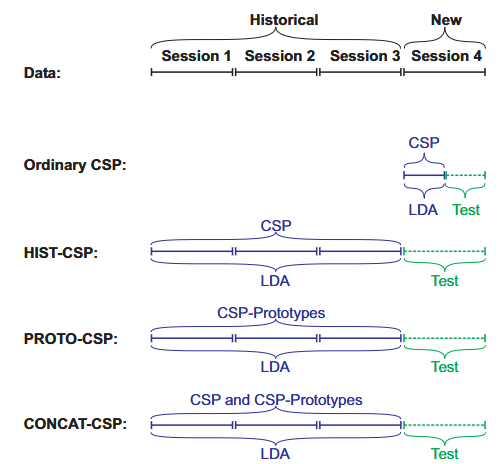
\includegraphics[scale=0.8]{gfx/MThes_CSPHistApproaches.png} 
    \caption{Overview over different CSP algorithm approaches using historical data from previous calibration (taken from \cite{krauledat-2007})}
    \label{rel:CSP_Hist}
\end{figure}

Results (visualized in Fig. \ref{rel:ZeroTrainErr}) show the classification error (in \%) of the individual CSP algorithm approaches used by Krauledat et al. using only historical data for training the classifier and proceeding directly to the feedback phase in new sessions. In contrast, the ordinary CSP approach still uses half of the session for calibration (as seen in Fig. \ref{rel:CSP_Hist}) and the rest of each new session for the feedback phase. The Zero-Training algorithms produced significantly low error percentages in most subjects, especially using the CONCAT-CSP approach, thus proving the feasibility of this approach for the reduction of calibration time of BCI.


\begin{figure}[H]
    %\hspace*{-1.0cm}
    \centering
    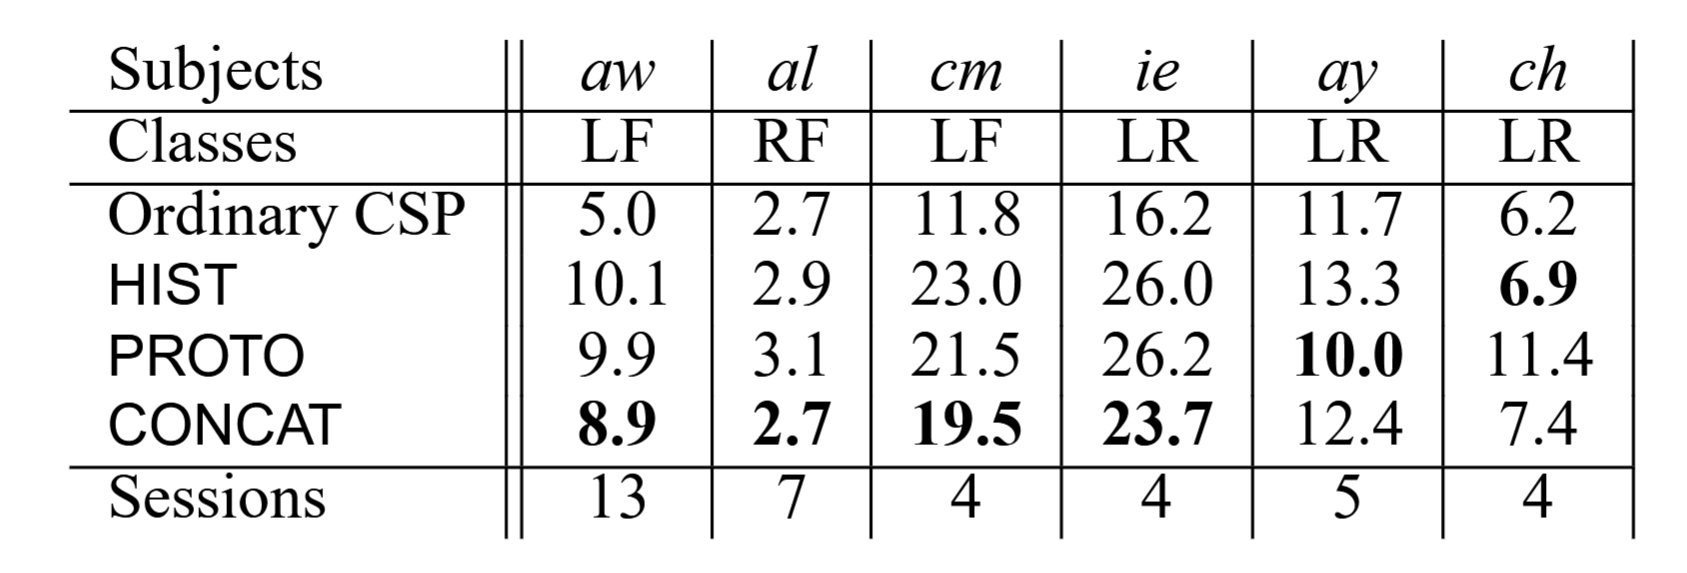
\includegraphics[scale=0.25]{gfx/MThes_ZeroTrainErrorProb.png} 
    \caption{Error rates (in \%) for the Zero-Training mode across the tested subjects with the error rate of the standard CSP as reference (taken from \cite{krauledat-2007})} % update description 
    \label{rel:ZeroTrainErr}
\end{figure}


A more recent study from the year 2022 seems to back up this method, albeit using a different approach in processing and using data of previously recorded data of individual test subjects for new BCI session for the exact same test subjects. % possibly rephrase
In their paper ``A Transfer Learning Algorithm to Reduce Brain-Computer Interface Calibration Time for Long-Term Users'' Giles et al. proposed a method of shortening calibration time for BCI sessions for long-term BCI users down to a few samples taken in each new session \cite{giles-2022}. To use the data from previous sessions, they suggest the use of their proposed r-KLwDSA Algorithm, consisting out of three steps (visualised in Fig. \ref{rel:rKLwDSA}):

% think aboiut if we should use a list or just paragraphs for now
\textbf{1. Data Space Alignment (DSA):} In this step the variance of the data from the previously recorded source sessions was reduced by applying a linear transformation to the recorded EEG data in order to align their data to the new session EEG data \cite{giles-2022} % maybe rephrase?
\newline
\textbf{2. Weighting:} Following that step, the aligned data was then compared to the new session's EEG data and weighted according to the similarities to the previously recorded data, making sure that the variance in data is further reduced by heavily weighing data that is similar to the data from the new session. This data is then used to calculate a covariance matrix of the previously recorded data, the ``transfer learning co-variance matrix'' % do we go more into detail about covariance matrix n stuff? + cite?
\newline
\textbf{3. Fusion:} The aligned data was then fused with the new session's EEG data using a regularization method proposed by Giles et al. which finds the optimal combination of existing and new EEG data by comparing validation accuracies of the individual combinations. Lastly, this data fusion was used to determine the Common Spatial Pattern (CSP) features within it to be able to train the BCI classifier

\begin{figure}[H]
    %\hspace*{-1.0cm}
    \centering
    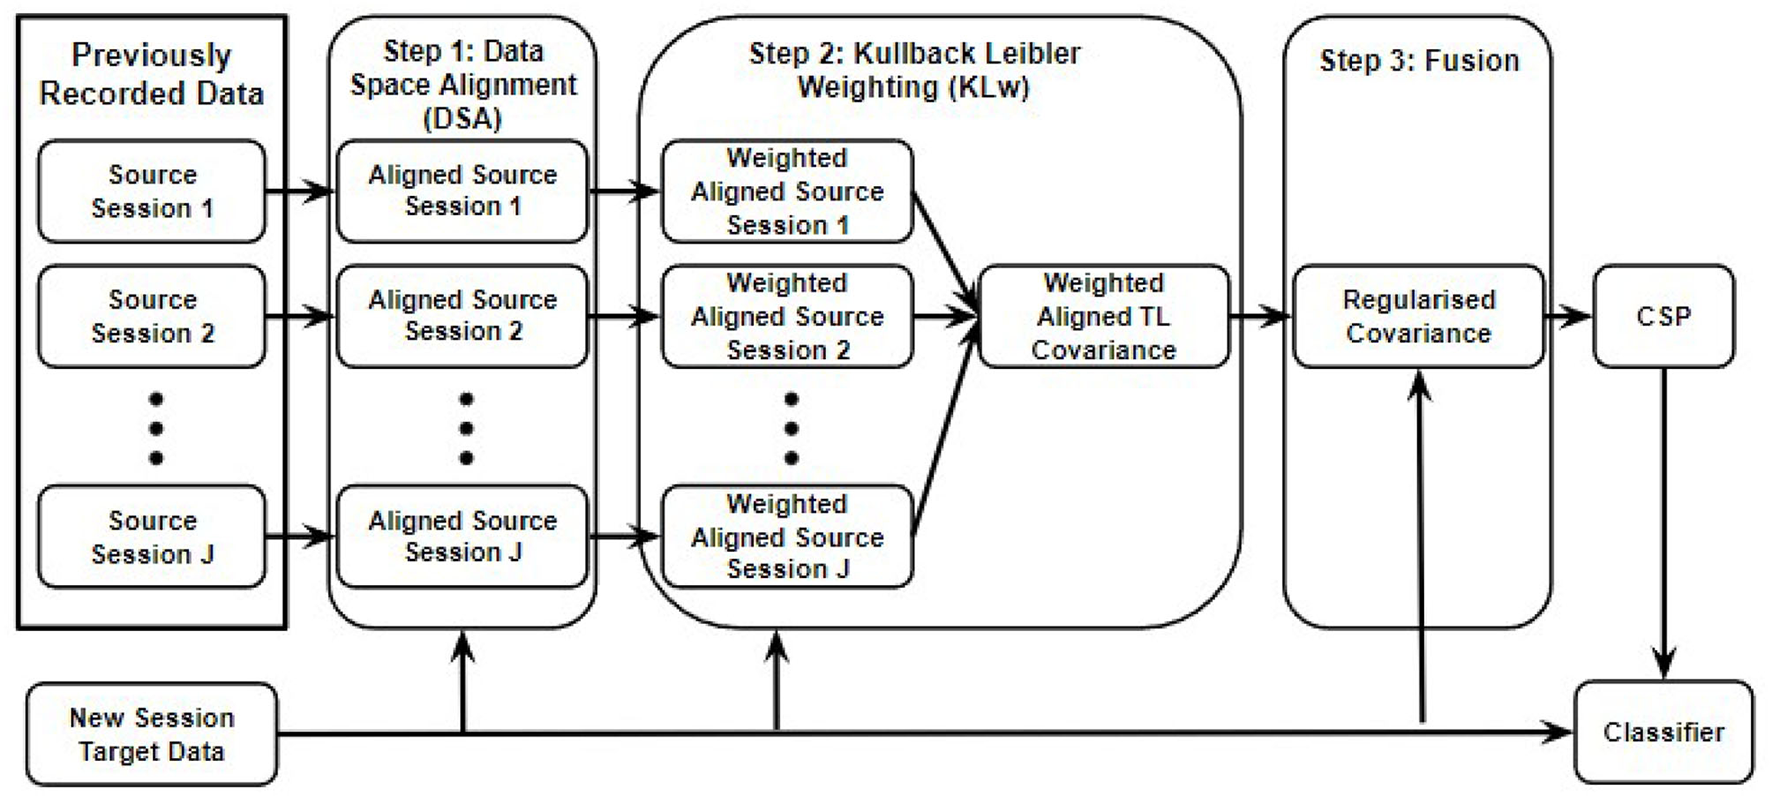
\includegraphics[scale=0.22]{gfx/MThes_rKLwDSA.png} 
    \caption{Overview over the proposed r-KLwDSA algorithm used in the paper of Giles et al. \cite{giles-2022}} % pdate description 
    \label{rel:rKLwDSA}
\end{figure}

Results showed that the proposed r-KLwDSA algorithm outperformed other approaches like using simple DSA or natural Transfer Learning in terms of average classification accuracy \cite{giles-2022}. % prob rephrase

Since, next to the previously mentioned inter-session variability, there is also a high inter-\emph{subject} variability of EEG data across recording sessions, algorithms that account for this variability are desirable for our presented use case. % do we actually mention it? Maybe reference + rephrase

While Kreuledat et al. and Giles et al. used the calibration data of previous BCI sessions of individual test subjects as a basis for removing the need of a calibration session for the exact same test subject, the approaches used in their work can serve as a foundation for an approach using previously recorded data of several different test subjects to shorten calibration time of new test subjects using BCIs, especially since the approaches using data alignment and transfer learning are practically the same for cross-session and cross-subject trasnfer learning \cite{wu-2020}. % rephrase? + mention that the general approach is similar and that the approaches were backed up by the review paper from 2020 by Xu n peeps


- mention CSP filters! (+ try to understand what they actually mean, might help to try to describe CSP in the definitions chapter before c:) [but don't go tooooo far into them, that's not your part in this thesis and doesn't really help our IT(!) (not neuroscience) focused reader group :33, keep it as detailed as needed, BUT! as simple as possible]

% ERD/ERS Event related synchonisation and desynchronsitation (!) Furthermore, it is known since Berger (1930) that certain events can block or desynchronize the ongoing alpha activity.(!) These types of changes are time-locked to the event but not phase-locked, and thus cannot be extracted by a simple linear method, such as averaging, but may be detected by frequency analysis. This means

% From paper:  The filtered signal corresponding to the desynchronization of the left hand motor cortex is characterized by a strong motor rhythm during imagination of right hand movements (left hand is in idle state), and by an attenuated motor rhythm during left hand imagination.
% -> Makes sense, as during thinking of left hand movement the region there is blocked/desynchronised, as it is being used :3

\section{Approaches using Neural Networks}
\label{sec:relWork:NN}

Algorithms, such as the ones presented in the previous chapter, use traditional machine learning and thus rely on an extensive feature extraction process to train a classifier (see for example Img. \ref{rel:rKLwDSA}). % rephrase image ref? + cite?
With the advancements made in the area of deep learning, approaches using Neural Networks can be considered for aiding the sought reduction of the calibration time. For this, according to a review paper on the use of deep learning techniques for classifying EEG Motor Imagery tasks by Altaheri et al. published in 2023, Convolutional Neural Networks (CNN) was the main architecture of Neural Networks used for the implementation of classifiers for said Motor Imaging tasks \cite{altaheri-2021}. Furthermore, the authors also pointed out the ability of the networks to work with raw data with minimal preprocessing to no preprocessing at all \cite{altaheri-2021}, significantly reducing the overhead of the algorithms in comparison to the machine learning approaches from the previous chapter which heavily rely on extensive preprocessing to align the highly variable datasets.% is that clear? Might write about specific papers for reduction of calibration time using CNN now (like 1 to 2 examplpes I guessss)      

An important discovery in this topic was made by Lawhern et al. in 2018, where the authors presented a special type of CNN that is specifically made to be used with EEG signals for Brain Computer Interfaces and is capable to classify EEG data for a multitude of BCI paradigms \cite{lawhern-2018}.% rephrase? 

\begin{figure}[H]
    %\hspace*{-1.0cm}
    \centering
    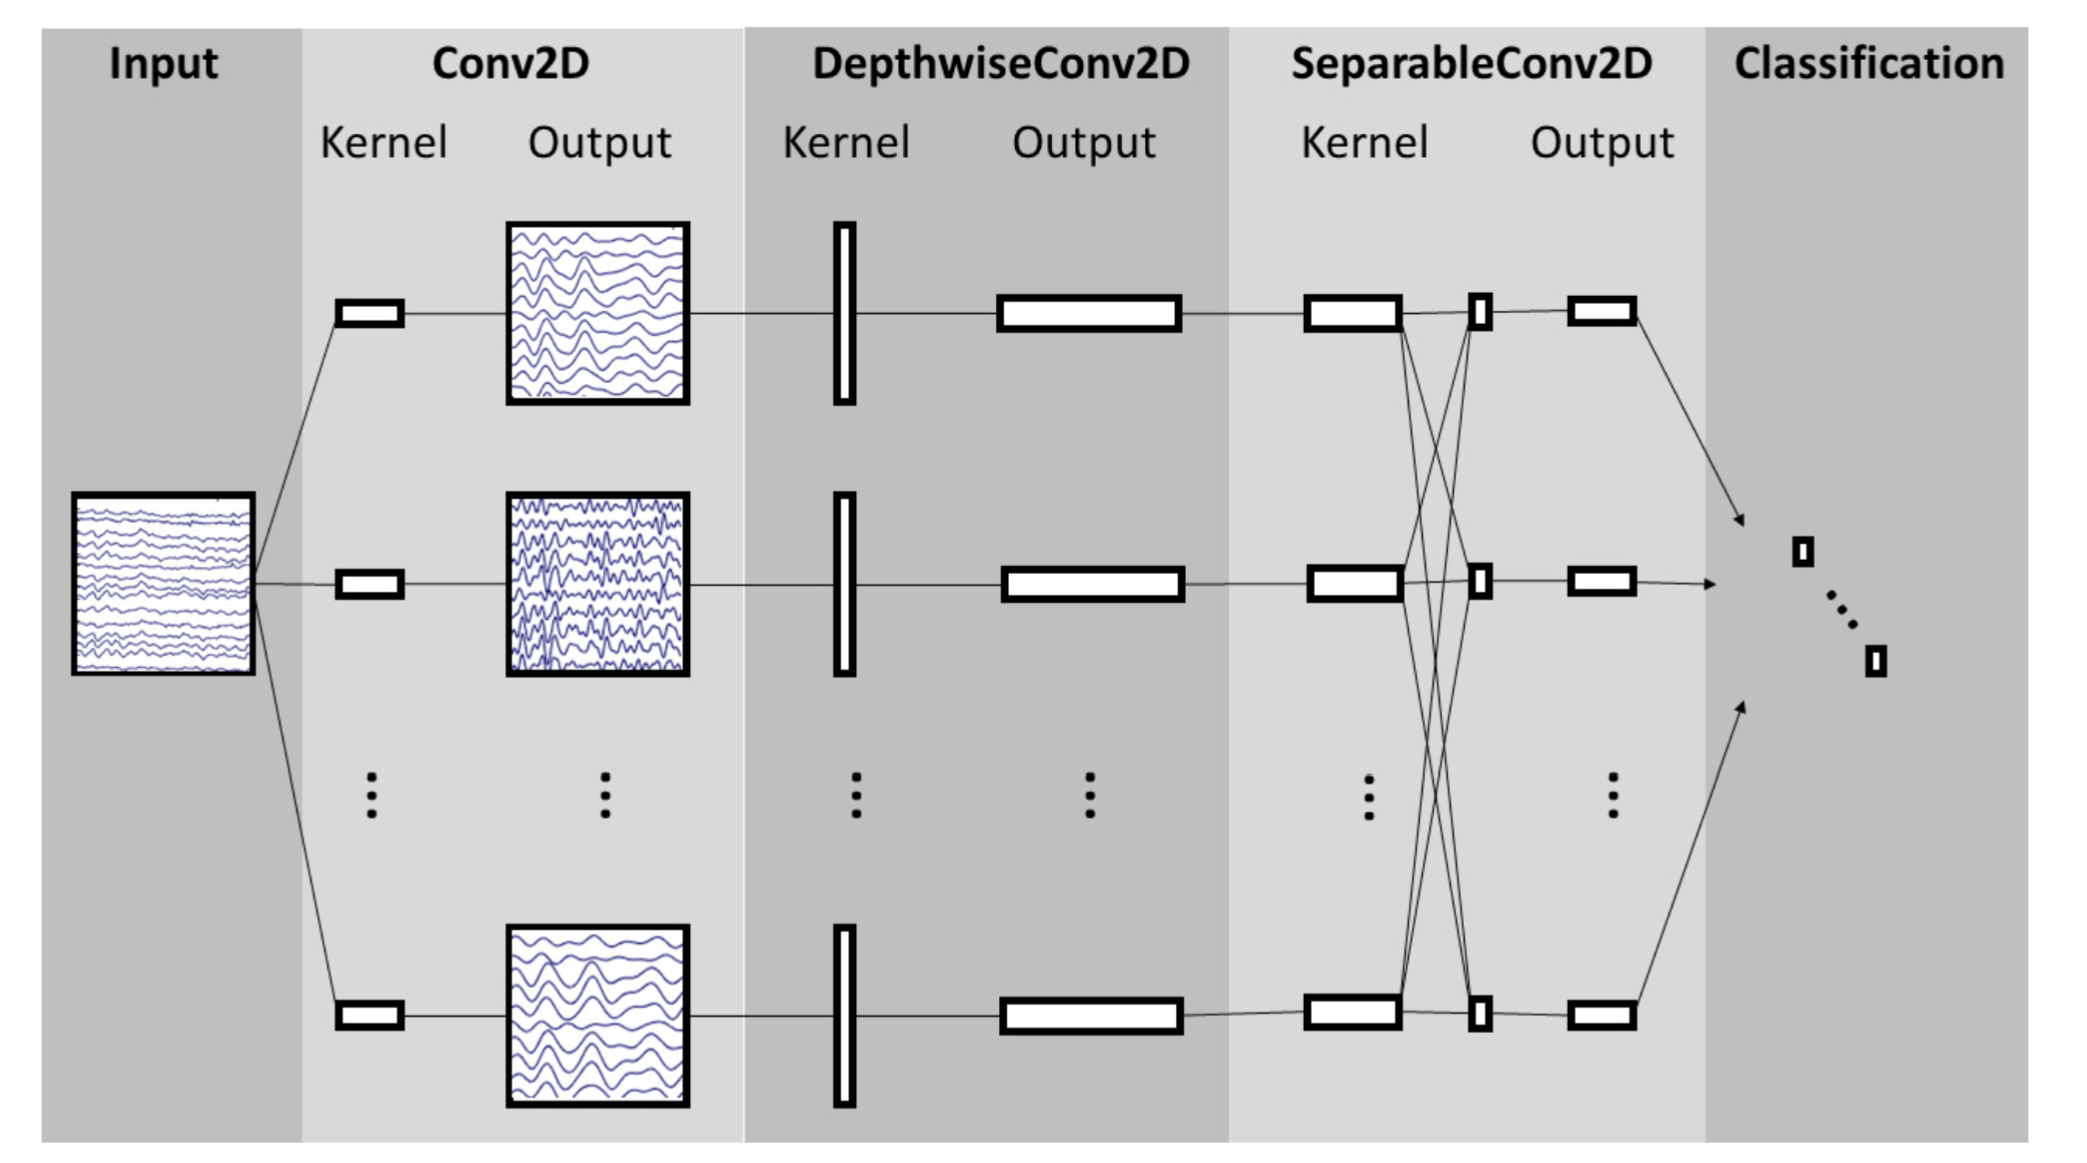
\includegraphics[scale=0.4]{gfx/MThes_EEGNetArchitecture.png} 
    \caption{Visualisation of the EEGNet architecture (taken from \cite{lawhern-2018})} % update description 
    \label{rel:EEGNetArch}
\end{figure}

The architecture of this network (see for reference Img. \ref{rel:EEGNetArch}) handles incoming EEG data as follows: % maybe think about converting this to a list at some point
First, the incoming data is temporally convoluted with a filter size of (1, 64), according to half of the sampling rate used in this paper, to enable the network to extract frequency information for the underlying data. The result of this convolution are feature maps containing EEG data for different frequency bands. % is that correct?
After that, another convolution is applied with a filter size of (n=numberOfChannels, 1) % reformat
which enables the network to extract spatial patterns for specific frequencies \cite{lawhern-2018}.Before the third convolution step, the sampling rate is reduced to 32Hz through an average pooling layer, after which the data is first convoluted with a filter of (1, 16), which represents 500ms of the recorded EEG activity, and then additionally convoluted convoluted pointwise with a (1, 1) filter. According to Lawhern et al. these two separated convolutions in the third convolution enable the network to separately learn to summarize the underlying feature map data in time, corresponding to the depth-wise convolution, and learn how to optimally combine these feature maps, corresponding to the point-wise convolution. Applied to the EEG signal, the authors describe that they first extract a 500ms ``summary'' of each available feature map before combining these summary outputs in the following step \cite{lawhern-2018}. % is that clear? Possibly rephrase (and look at the picture description)                         
% do we put this (from chatgpt) in here too? 
% Overall, the architecture is specifically designed to mimic traditional EEG feature extraction methods such as filter-bank CSP while leveraging the efficiency and flexibility of convolutional neural networks.
A reference of the detailed list of the individual layers used for the EEGNet can be found in the appendix under Img. \ref{app:EEGNetDetail}, which also shows sizes, number of parameters, outputs and possible options depending on layer. % is that clear?

% description from the image of the paper of the architecture: The network starts with a temporal convolution (second column) to learn frequency filters, then uses a depthwise convolution (middle column), connected to each feature map individually, to learn frequency-specific spatial filters. The separable convolution (fourth column) is a combination of a depthwise convolution, which learns a temporal summary for each feature map individually, followed by a pointwise convolution, which learns how to optimally mix the feature maps together. Full details about the network architecture can be found in Table 2

To prove the performance of the EEGNet, the validation accuracy of this network across different BCI paradigms, such as the SMR paradigms which is relevant to our thesis subject, was assessed and compared to other CNN architectures. % are they really all CNN archtiecturres?
A total of two configurations of the EEGNet, ``EEGNet-4,2'' and ``EEGNet-8,2'', were used for testing where the 4 and 8 denote the amount of temporal filters learned during training while the 2 indicates the amount of spatial filters learned per temporal filter \cite{lawhern-2018}.
While the EEGNet showed consistently high validation accuracies for paradigms such as P300 ($>=90\%$)% do we mention the different paradigms in the beginning? of this section? Nmely the four paradigms used in this study
for both inter-subject and cross-subject classification, the EEGNet showed significantly lower validation accuracy for the SMR paradigm for inter-subject and cross-subject classification (see Img. \ref{rel:EEGNetSMRAcc}) compared to other BCI paradigms. % is that clear
Still, the EEGNet consistently matched or outperformed other CNN network architectures in terms of validation accuracy on the individual paradigms and can thus be used as a basis for an approach of lowering calibration time needed for BCI using neural networks. % is that clear? or is that closing this chapter 'too soon?'

\begin{figure}[H]
    %\hspace*{-1.0cm}
    \centering
    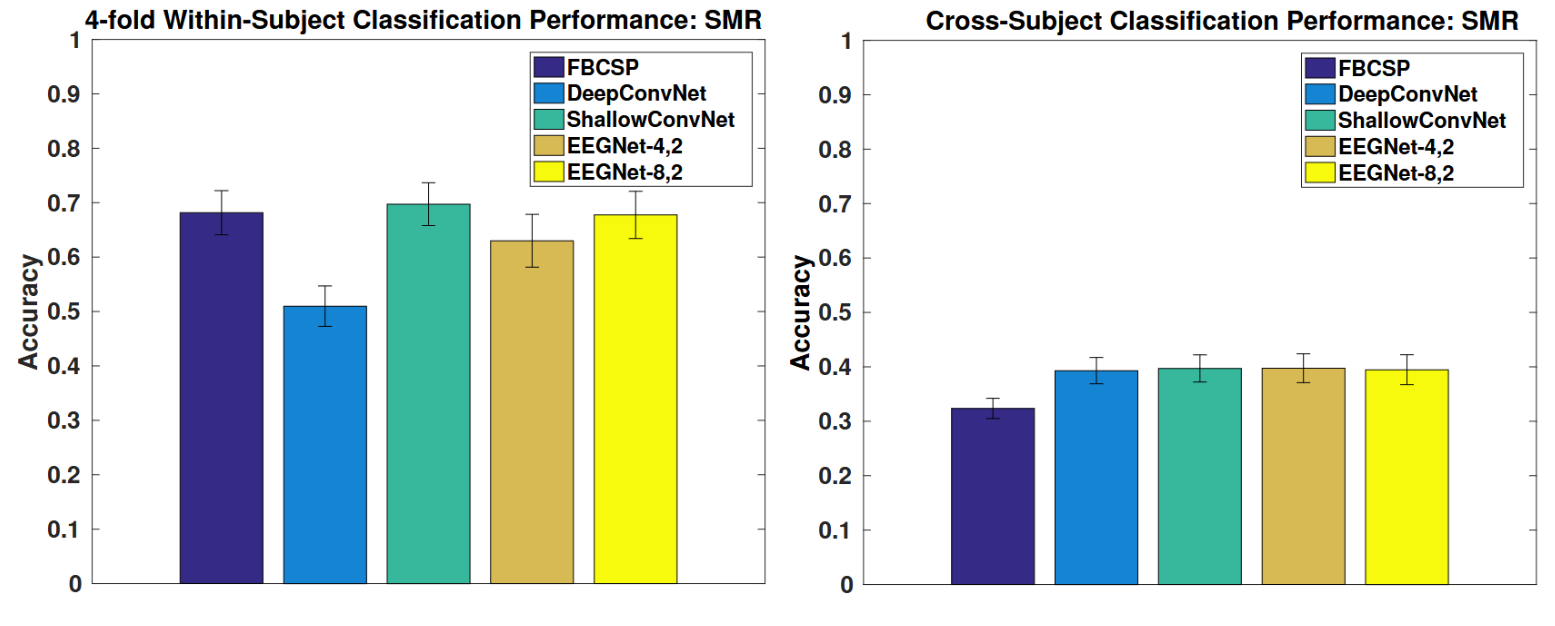
\includegraphics[scale=0.35]{gfx/MThes_EEGNetSMRAcc.png} 
    \caption{Comparison of validation accuracies of the presented EEGNet to other network architectures on both Withing-Subject and Cross-Subject classification (taken from \cite{lawhern-2018})} % update description + explain what 8,2 and 4,2 means c: 
    \label{rel:EEGNetSMRAcc}
\end{figure}

An important strength of the presented network is that it is able to generalize well both while classifying EEG data from the same subject as well as data from different subjects, leveraging the underlying problem of having high inter-session and inter-subject variance of EEG data, which the ML approaches in the previous section tried to address. % rephrase?
Furthermore, the EEGNet proves to be usable for a wide range of BCI paradigms, both ERP, like P300 and SSVEP, and SP like the mental commands performed in task like MI \cite{lawhern-2018}. % rephrase + adjust to recently written results section

Since the publication of this paper in 2018, new and improved architectures of neural networks for classification of EEG data were presented which also show increased validation accuracies for Motor Imaging \cite{salami-2022, wei-2024}. % will we get into detail here? (have tried before but was too complex to go into detail)


% put the detailed layer list into the appendix c:
More recently, in the paper ``Cross-subject EEG Decoding with spatiotemporal transformers for
zero-calibration brain–computer interfaces'' published in 2026, Jiang et al. propose a network based on the architecture of transformers % reference to grundlagen chapter? C:
that is able to accurately classify for Motor Imagery tasks without the need of prior calibration \cite{jiang-2026}, which accurately fits our use case of having a multitude of players use a BCI without prior experience and recorded BCI sessions.  
% chatgpt stuff to maybe add: In contrast to traditional CNN-based approaches, which mainly focus on local spatial–temporal patterns, the transformer architecture is designed to capture long-range dependencies and relationships within EEG signals through self-attention mechanisms \cite{bci-transformer-2026}.

\begin{figure}[H]
    \hspace*{-0.5cm}
    \centering
    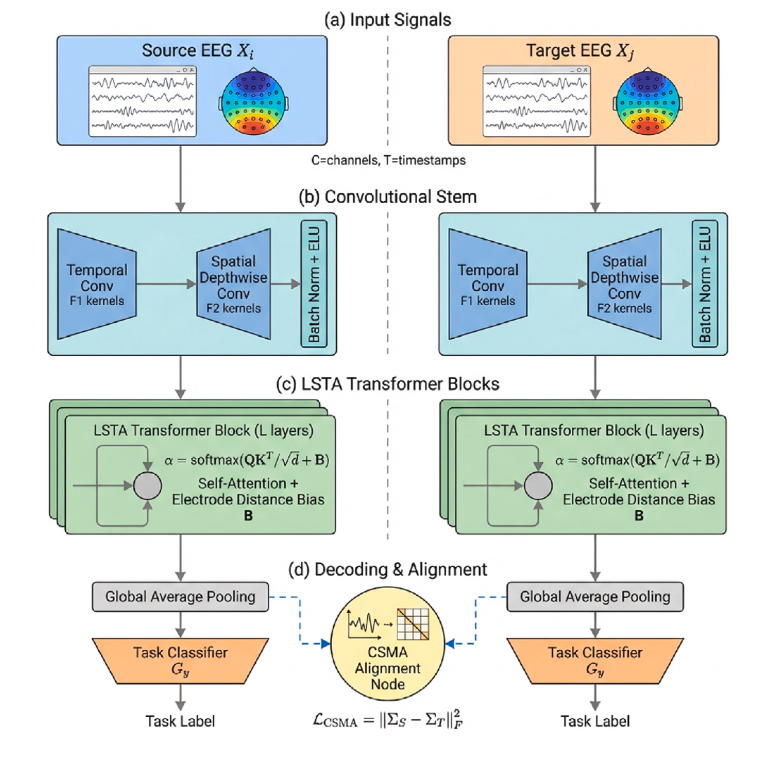
\includegraphics[scale=0.45]{gfx/MThes_BCITransArch.png} 
    \caption{Overview of the BCI-Transformer architecture featuring a dual-stream approach for the source and target EEG data and, LSTA transformer block, and parallel flow through the classifier and the CSMA node (taken from \cite{jiang-2026})} % shorten image description?
    \label{rel:BCITransArch}
\end{figure}

% also mention that it is a hybrid between CNN and tranformer architecture
The hybrid architecture of the proposed network (shown in Img. \ref{rel:BCITransArch}) uses both a classic CNN for spatial and temporal feature extraction and so-called ``Localized Spatiotemporal Attention'' transformer blocks. These blocks focus attention on physiologically relevant electrodes like the electrodes around the motor cortex for MI tasks, compared to classic attention mechanisms in transformers that would attend to all available channels\cite{jiang-2026}. % rephrase?
This initial focus, which can be overridden and is adapted in relation to discovered subject-independent pattern during learning, additionally allows the LSTA blocks to lower subject-specific artifacts in the recorded EEG signals \cite{jiang-2026}.



% now explain the other important step mentioned in the paper :3
Additionally, the network features a Cross-Subject Manifold Alignment (CSMA) node, which aligns the feature spaces of the individual subjects into one shared feature space \cite{jiang-2026}. This reduces distribution shifts and helps the network to learn subject-invariant patterns in the recorded EEG data while still preserving the ability to distinguish between individual classes in the shared feature space \cite{jiang-2026}. % clear? (should be, I think)   
- CSMA (Cross-Subject Manifold Alignment)
% in words of author:  Cross-Subject Manifold Alignment: We define a novel manifold alignment objective (CSMA) that minimizes the discrepancy between the second-order statistics of the latent representations of different subjects, projecting diverse neural distributions into a shared, class-discriminative geometric space.

% in words of chatgpt: The \textbf{Cross-Subject Manifold Alignment (CSMA)} component is used to reduce the variability between different users by projecting EEG data from multiple subjects into a shared latent feature space. Through this alignment process, the model learns subject-invariant representations while preserving class-specific information required for classification. As a result, EEG data from different users becomes more similar in distribution, enabling the classifier to generalise better to unseen subjects without requiring extensive


To prove the performance of the BCI-Transformer, the network was tested on three EEG datasets for Motor Imagery % do we need details? (might ask Guthe)
for zero-calibration capability, representing a possible cross-subject application of the BCI. Results showed that the proposed BCI-Transformer outperformed all 22 networks, across all three datasets, it was compared against achieving validation accuracies 77\% to 88\% depending on the dataset. While the complexity and inference time of the BCI-Transformer was higher than other existing architectures like the EEGNet \cite{jiang-2026}, the achieved validation accuracy of the network in zero-calibration scenarios could outweigh the computational effort needed to use this network architecture. % rephrase?
% append results table into the appendix instead of showing it here?
%  (+ ask pipp how he added an appendix, just to be sure)

This chapter has shown approaches for reducing calibration time through using data recorded from previous sessions (see Sec. \ref{sec:relWork:TL}) and using specific neural network architectures for classifying EEG data without the need of any prior calibration for new users. Therefore, this chapter can serve as proof and support of the possibility of finding approaches that significantly decrease the calibration time needed for new players to be able to use a BCI in video games, which are presented in detail in the following chapter. % passt formulierung so? 


% spatial features -> where is the EEG signal detected
% temporal features -> when is the EEG signal detected?

% also might think if we incorporate some stuff with data augmentation or if we just mention this in our approaches as an obvious way to increase the data we ahve for training (not sure we'd need to describe this in our grundlagen chapter)
% don't think so actually :3 if we need it we'll just mention it in our approach c: